\documentclass[12pt]{article}
\usepackage[utf8]{inputenc}
\usepackage[T1]{fontenc}
\usepackage[spanish]{babel}
\usepackage[a4paper,left=3cm,right=2cm,top=2.5cm,bottom=2.5cm]{geometry}
\usepackage{lmodern}
\usepackage{graphicx}
\usepackage{graphics}
\usepackage{color}
\usepackage[hidelinks]{hyperref}
\usepackage[makeroom]{cancel}
\usepackage{amsmath}
\usepackage{enumerate}
\usepackage{amssymb}
\usepackage{amsfonts}
\usepackage{float}
\usepackage{epstopdf}
\usepackage[table]{xcolor}
\usepackage[final]{pdfpages}
\usepackage{float}
\usepackage{fancyhdr}
\pagestyle{fancy}
\fancyhf{}
\lhead{Sistemas electrónicos}
\rhead{Jorge Benavides Macías}
\rfoot{\thepage}
\renewcommand{\headrulewidth}{0.4pt}% Default \headrulewidth is 0.4pt
\setlength{\headheight}{16pt}
\setlength{\parskip}{1em}
\setlength{\parindent}{0em}
%\renewcommand{\baselinestretch}{1.5}
\begin{document}
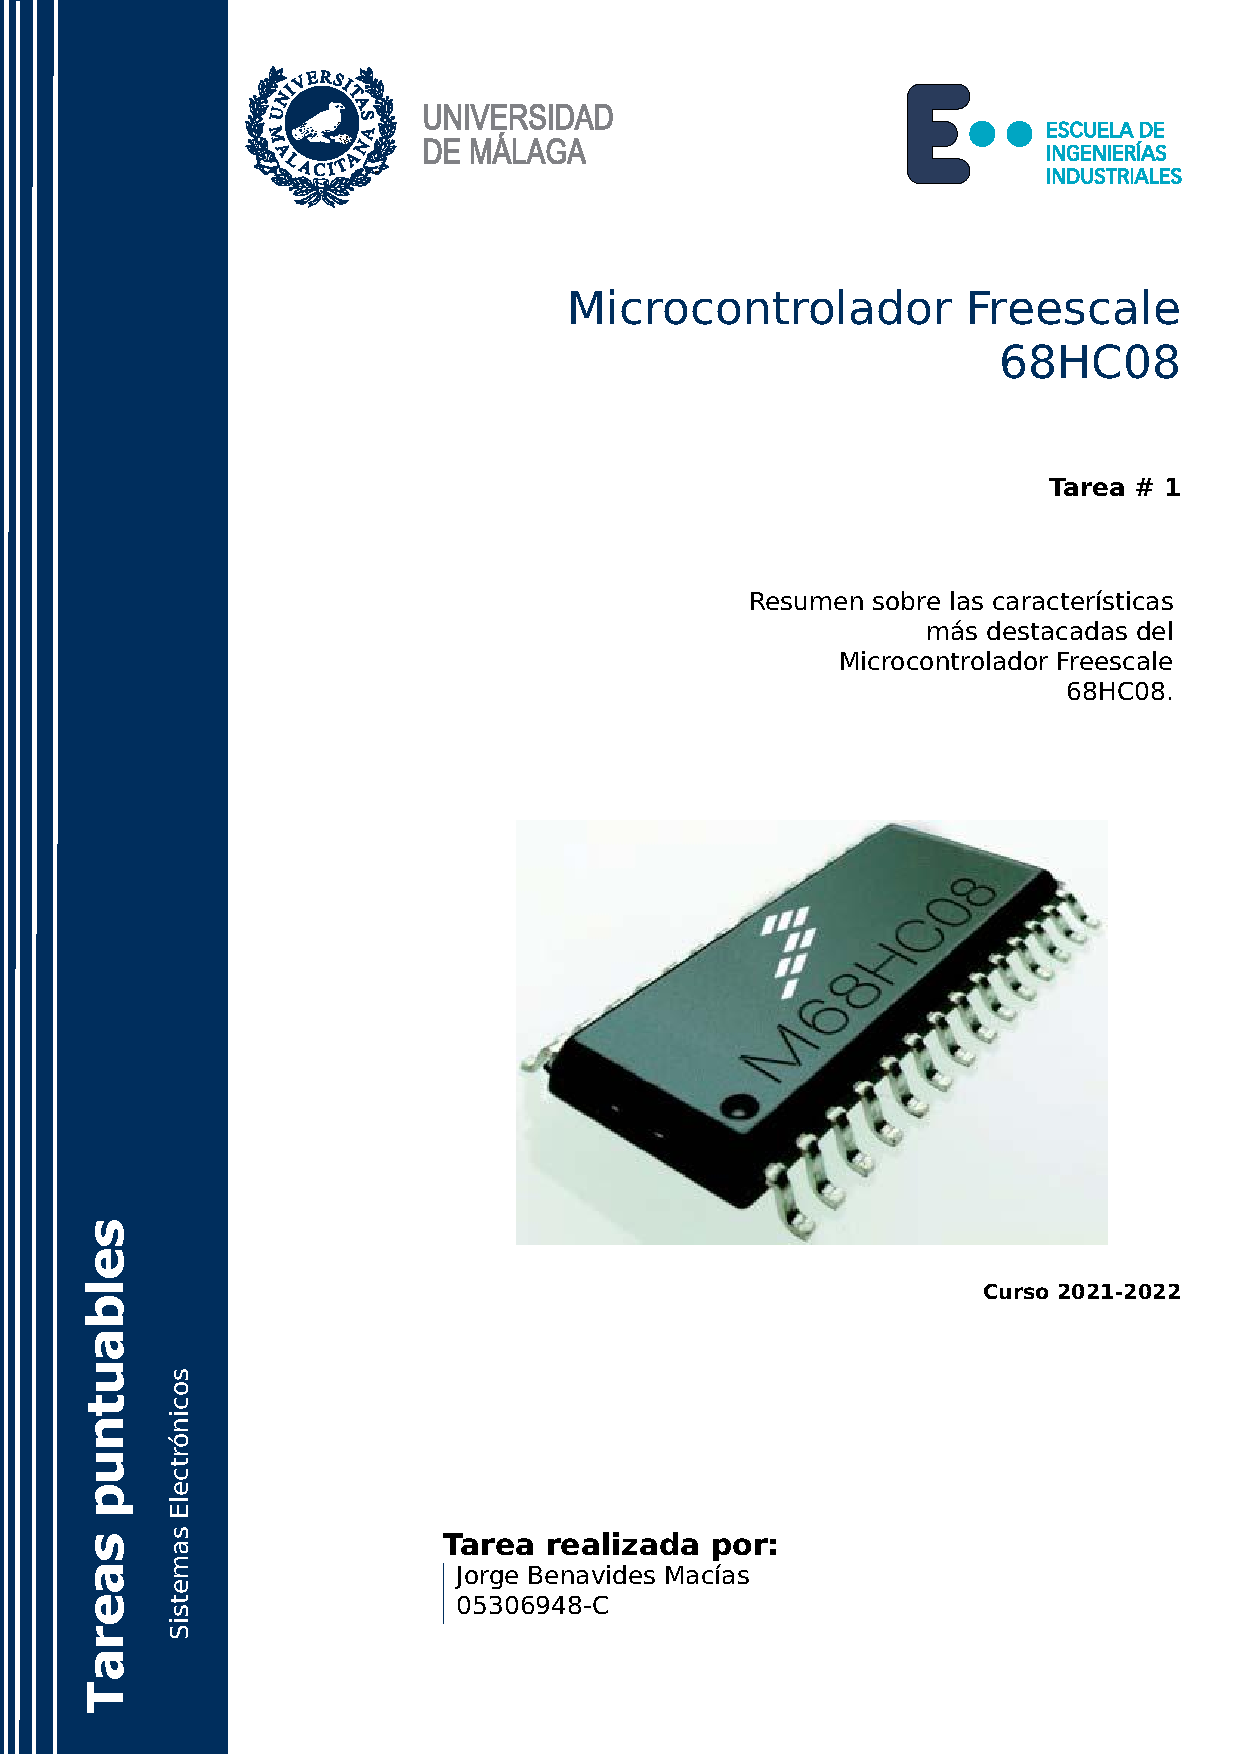
\includepdf[pages=-]{Portada_tarea_Jorge}
El microcontrolador Freescale 68HC08 es un microcontrolador de propósito general\footnote{Sus características pueden resolver un rango muy amplio de tareas.} que pertenecía a Motorola y tiempo después fue adquirido por Freescale Semiconductor. Su unidad de procesamiento, la \textbf{CPU08}, permite que el ``código objeto'' del microcontrolador 68HC05 sea compatible con el 68HC08, lo cual aumenta el rendimiento sin inversión de tiempo ni de software.

{\large{\textbf{CPU}}}

Dado que el CPU08 es el núcleo de nuestro microcontrolador es necesario describir ciertos aspectos importantes de trabajo por ejemplo: 
\begin{itemize}
    \item El tiempo de ejecución:
    Un ciclo de cada ejecución equivale a 4 fases del reloj, es decir un cuarto de la frecuencia del reloj, además incluye un PLL\footnote{Sistema de control para sincronizar señales.} interno para generar el reloj de referencia.
    \item Arquitectura: Presenta una arquitectura \textbf{Von Neumann} y cuenta con 64Kbytes de trabajo que se reparten entre la RAM, ROM o Flash, Vectores, el programa monitor, los registros de control y una zona de memoria no accesible que tiene como objetivo comprobar direcciones ilegales, esto permite resolver errores sin afectar los datos ya guardados.
    \begin{figure}[h]
        \centering
        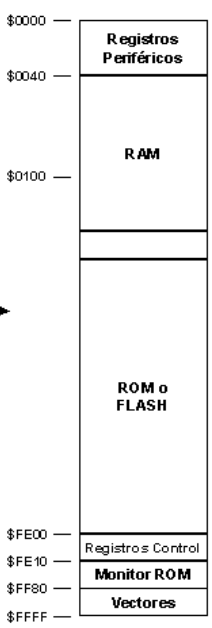
\includegraphics[scale=0.5]{esquema de memoria .png}
        \caption{Distribución de la memoria}
        \label{fig:memory_distribution}
    \end{figure}
    \item Instrucciones: Tiene un  total de 85 instrucciones, 28 son nuevas respecto a la versión anterior 68HC05, muchas de ellas soportan el registro del índice extendido a 16 bits y el puntero de pila se puede recuperar.
    \item Modos de direccionamiento: Inherente, Inmediato, Directo, Extendido, Indexado\footnote{sin offset, sin offset con incremento posterios,con offset de 8 bits, con offset de 8 bits con incremento posterior,con offset de 16 bits.}, stack pointer con offset de 8 y 16 bits, relativo y memoria a memoria. Cada uno de estos modos permite direccionar tablas y estructuras eficazmente, lo que se traduce en ejecutar instrucciones más rápido y eficientemente.
\end{itemize} 

{\large{\textbf{Módulo del Reset y las interrupciones}}}

Este módulo es de suma importancia y ofrece una gran ventaja frente a otros dispositivos que no lo poseen ya que permite gestionar solicitudes (generalmente hechas por periféricos) asíncronas sin comprometer la ejecución del programa inicial. 

El \textit{reset} restaura al dispositivo a un estado conocido, que generalmente es la primera instrucción junto con la carga del PC. 

Las interrupciones son similares al \textit{reset}, ya que envían al microcontrolador a un estado conocido que gestione la solicitud sin perder el estado actual del PC, para recuperarlo y continuar la ejecución del programa principal. El CPU08 puede gestionar hasta 128 interrupciones descontando el \textit{reset} e interrupciones de software por lo tanto quedan 126 interrupciones libres para los periféricos; es importante destacar que las interrupciones tienen prioridades y la más alta la tiene el SWI (interrupciones de software).


{\large{\textbf{Módulo ADC}}}

Algunas unidades de esta familia poseen un convertidor de 8 o 10 bits de resolución. Generalmente soportan dos modos de conversión, el modo de conversión continua donde la entrada del ADC se convierte continuamente y se guarda en el registro sin importar los datos anteriores, el otro es el modo de conversión única que completa un conversión entre escribir el registro de estado y el de control.

{\large{\textbf{Módulo SCI}}}

También llamado UART (Universal Asynchronous Receiver Transmiter) permite la comunicación con otros dispositivos u otro microcontrolador en tres modos distintos: full-duplex, asíncrono y alta velocidad. Este módulo trabaja con dos tipos de longitudes (8 o 9 bits).

{\large{\textbf{Módulo Varios}}}

Módulo COP (Computer Operating Properly): Es un contador que corre libremente, el usuario puede modificarlo y permite recuperarse de eventos inesperados.

Módulo LVI (Low Voltage Inhibit): Protege al sistema durante una caída de alimentación mediante un reset.

Módulo TIM (Timer Interface Module): Funciones varias como comparación de salida, captura de entrada y modulación de ancho de pulso.


{\large{\textbf{Conclusión}}}

Es un microcontrolador de uso general, de bajo costo, con múltiples aplicaciones (juegos retro o afinadores), que por su gran abanico de módulos cubre todo tipo de necesidades como la comunicación interna y externa con otros dispositivos, periféricos útiles que permiten ahorrar en componentes, su amplio juego de instrucciones y por supuesto sus recursos de protección del sistema.

\end{document}